\documentclass{beamer}	
\mode<presentation>
 
\usepackage{pdfpages}
\usepackage{fancyvrb}

\usepackage{amsmath}		%% mathematics typesetting
\usepackage{amssymb}
 
\usepackage{epigraph}   %% nice setting of quotations

\usepackage{tabularx} %% allows to use row colours in tables

\usepackage{ulem}

\usepackage{booktabs}

\usepackage{siunitx} %% tpyeset SI units

\usepackage{CJKutf8} %% typeset Chinese characters

\usepackage{pdfpages}%% include pdfs

\usepackage{subfigure}

\usepackage{animate} %% show animated gifs

\DeclareMathAlphabet{\mathcalligra}{T1}{calligra}{m}{n}

\newcommand{\heart}{\ensuremath\heartsuit} % make a heart if needed

% Color and Theme. Can be changed. However, this one's quite nice.
\usetheme{Madrid}
\definecolor{theme}{rgb}{0.84,0,0.21}
\usecolortheme[named=theme]{structure}


%%  Title information
\title[Daten erheben und darstellen]{M14.6 Daten erheben und darstellen}
\author[melanie.stefan@medicalschool-berlin.de]{M14 Wissenschaftliches Arbeiten}
\institute[]{Prof. Melanie Stefan - melanie.stefan@medicalschool-berlin.de}
\date[]{letzte Änderung: WS 2024/25} 

% Table of contents to pop up at the beginning of each section
\AtBeginSection[]
{
  \begin{frame}<beamer>
    \frametitle{Outline}
    \tableofcontents[currentsection,currentsubsection]
  \end{frame}
}

\AtBeginSubsection[]
{
  \begin{frame}<beamer>
    \frametitle{Outline}
    \tableofcontents[currentsection,currentsubsection]
  \end{frame}
}

 
\beamertemplatenavigationsymbolsempty

\begin{document}
 
  { \usebackgroundtemplate{
\includegraphics[width=1.2\paperwidth]{MSB_Titelseite.pdf}} 
\begin{frame}

 \maketitle 

$\,$\\[6cm] 

\end{frame} 
}


%% Hook
\begin{frame}{Was mache ich mit Daten?}

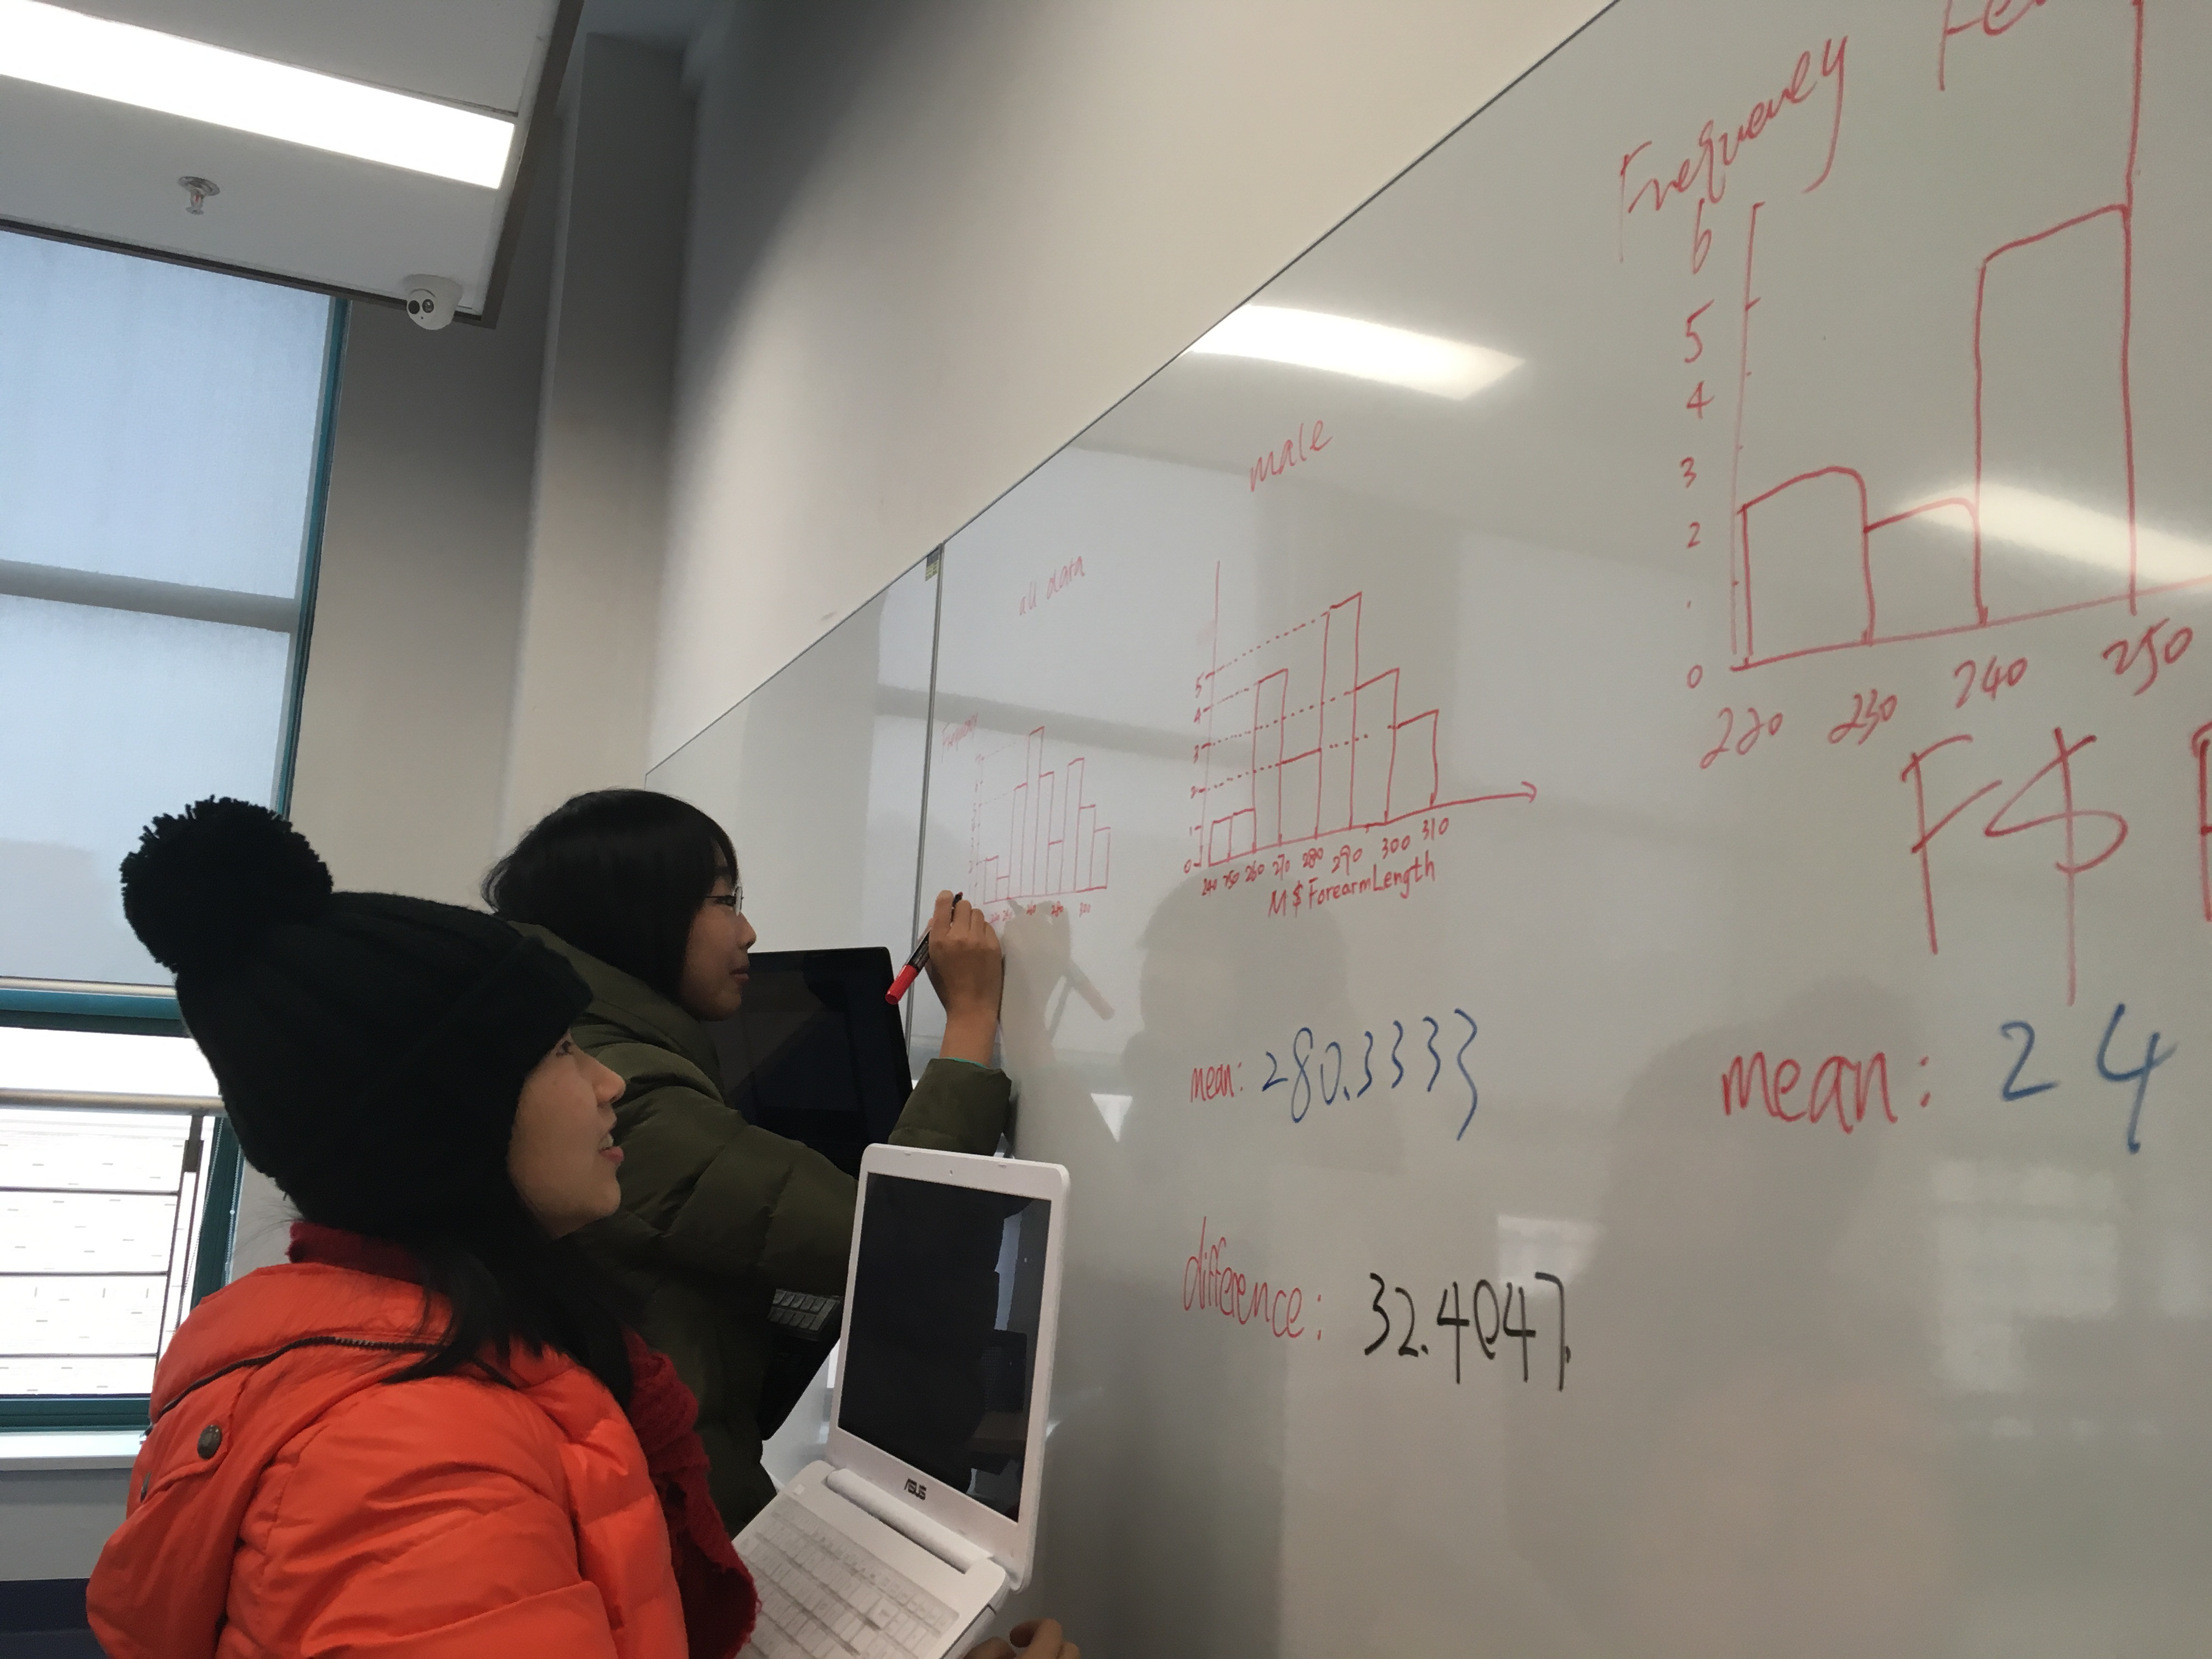
\includegraphics[width=\textwidth]{students_drawing_histograms.jpg}
    
\end{frame}


%% TLIA
\begin{frame}{In dieser Vorlesung geht es darum, Datensätze \dots}

\begin{columns}[c]
\begin{column}{5cm}

\begin{itemize}
    \item 
    \dots sauber zu erheben
    \item 
    \dots mit anderen zu teilen
    \item 
    \dots zusammenzufassen
    \item 
    \dots zu visualisieren
\end{itemize}

\end{column}

\begin{column}{5cm}
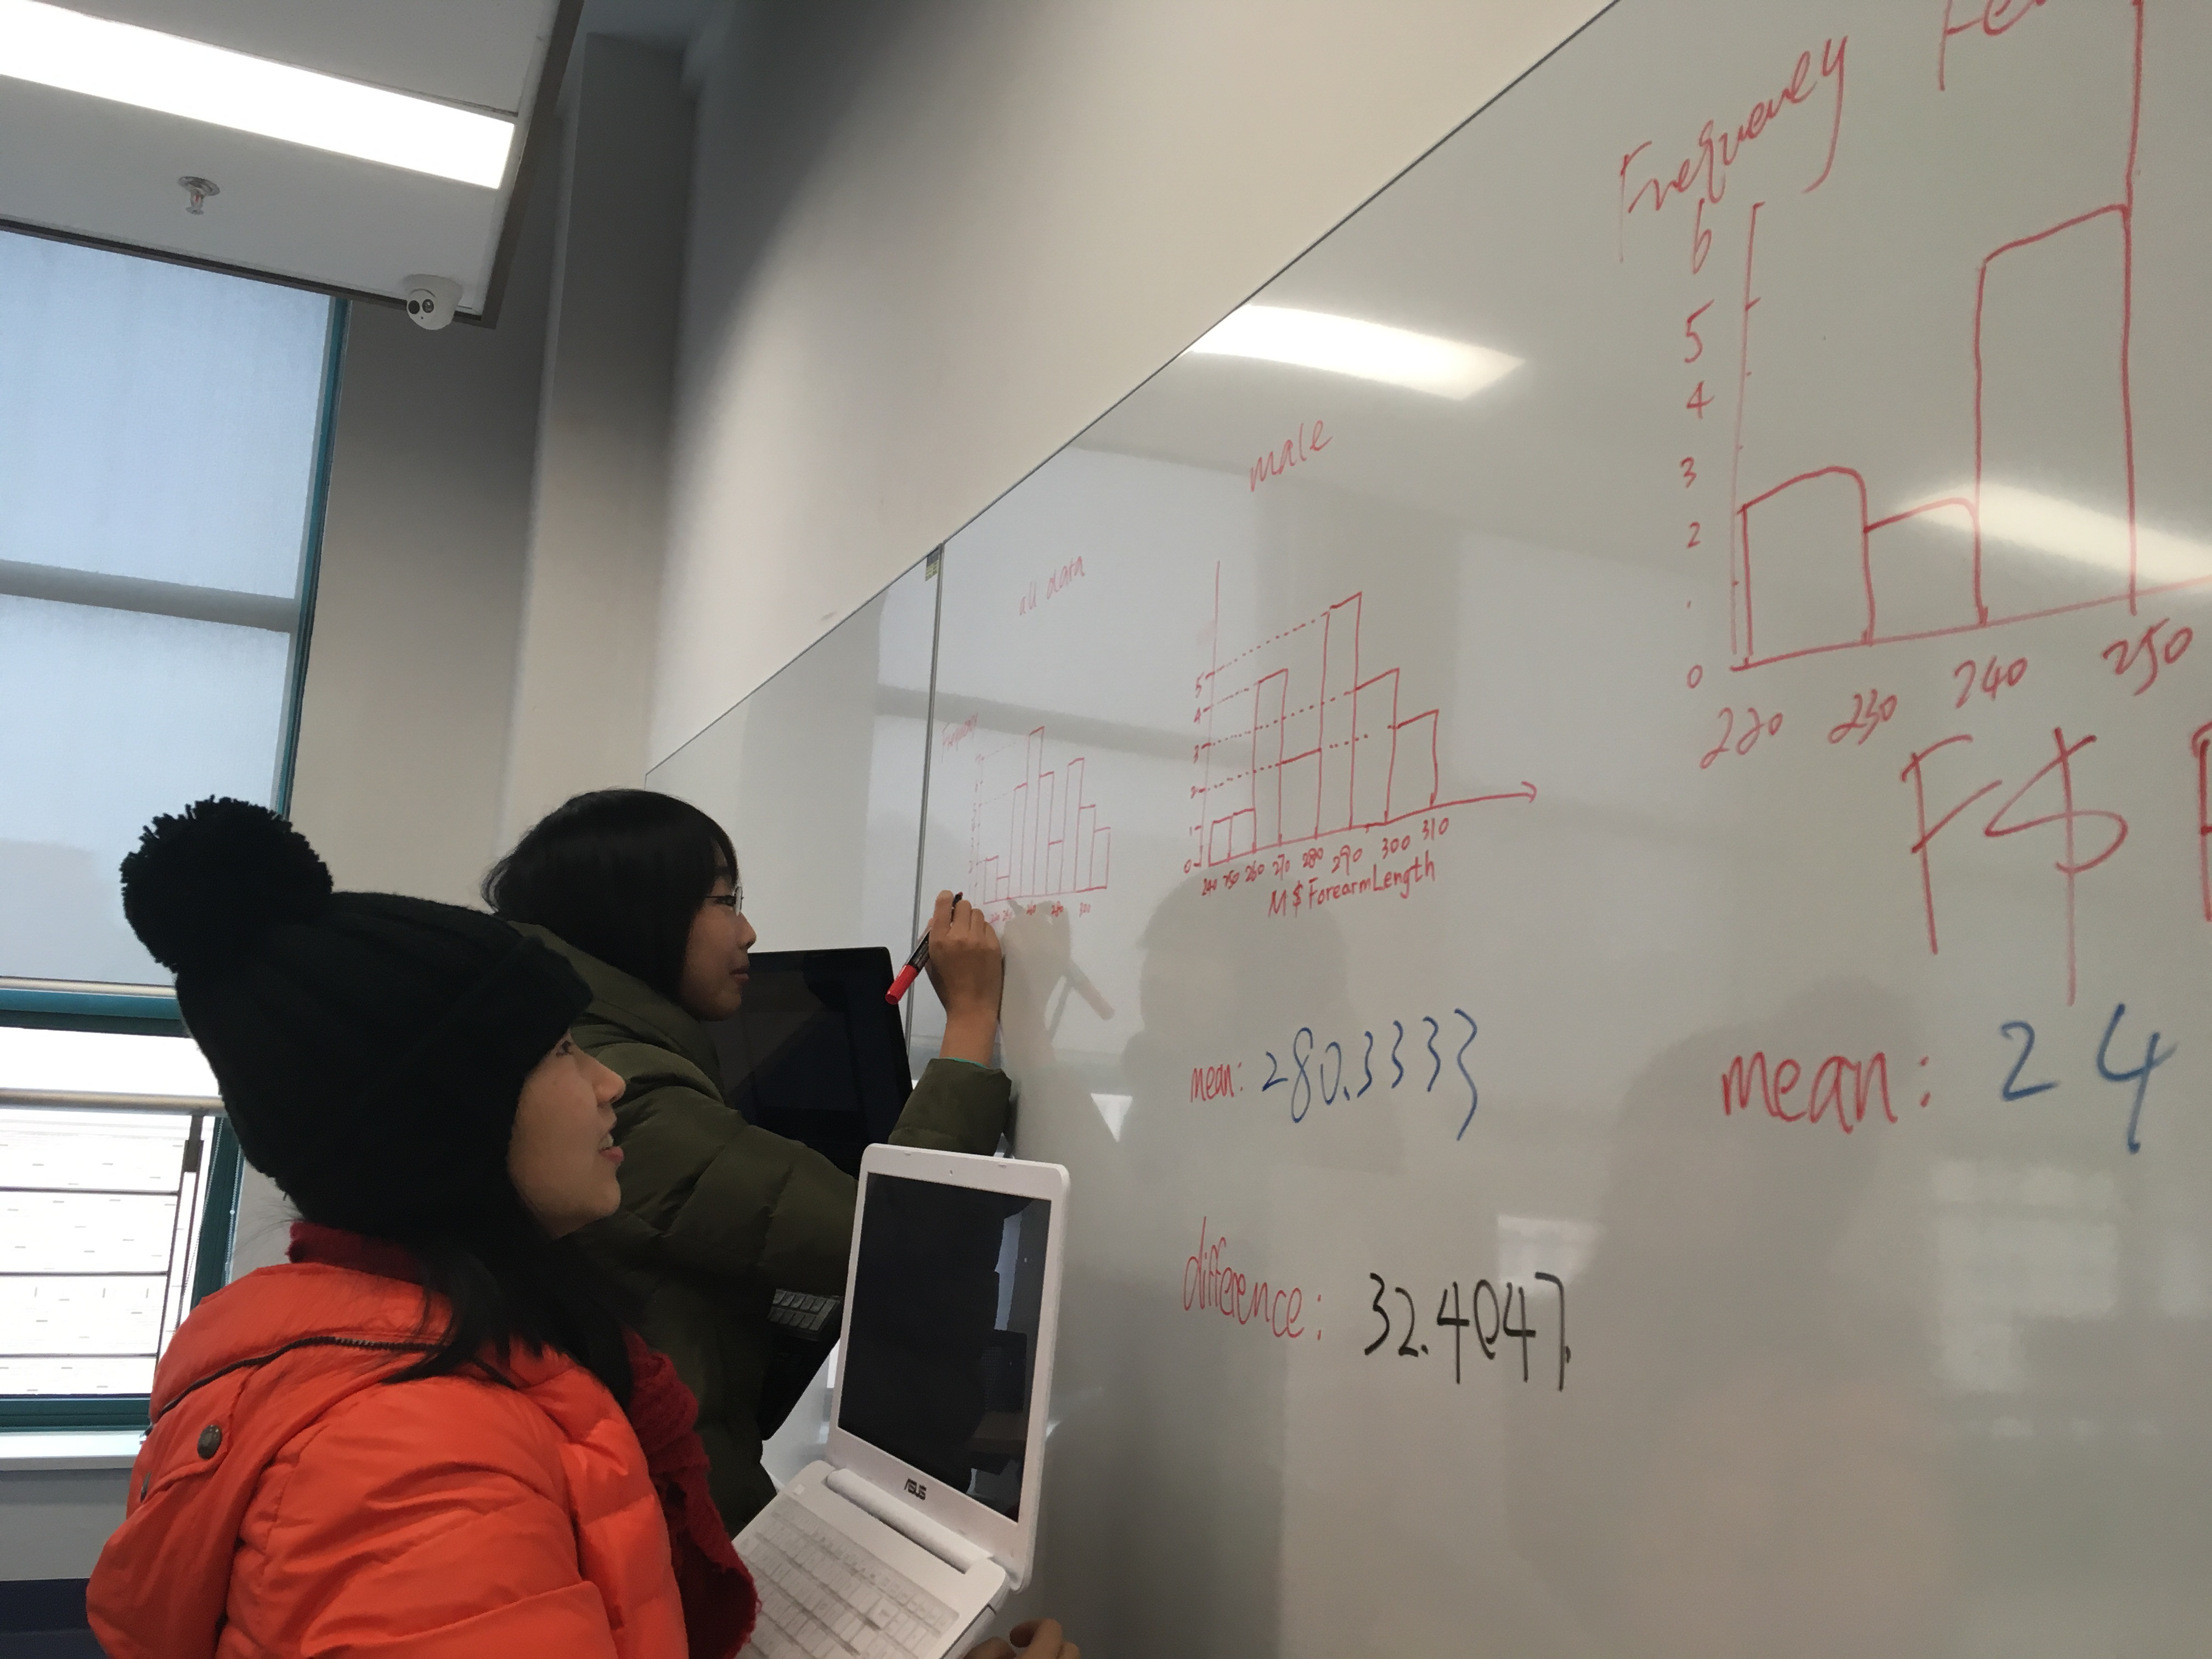
\includegraphics[width=\textwidth]{students_drawing_histograms.jpg}

\end{column}


\end{columns}


\end{frame}


%% Learning Objectives
 
\begin{frame}

\frametitle{Nach dieser Vorlesung sollten Sie:}



\begin{block}{Wissen:}

%%%%%
\begin{itemize}
\item
Erklären, was der Begriff "tidy data" ("saubere Daten") bedeutet
\item 
Beschreibende Statistiken (arithmetisches Mittel, Standardabweichung, Median, IQR, Modalwert) definieren
\item 
Häufige Verfahren zur visuellen Darstellung von eindimensionalen Daten (z.B. Histogramme, Box Plots) benennen und beschreiben 
\end{itemize}

\end{block}

 


\end{frame}

\begin{frame}

\frametitle{Nach dieser Vorlesung sollten Sie:}


\begin{block}{Können:}
\begin{itemize}
\item
Eine Datenerhebung sauber durchführen und protokollieren
\item 
Einen Datensatz säubern
\item
Häufige Visualisierungen von Daten (z.B. Histogramme, Box Plots) interpretieren
\item
Die Visualisierung von Datensätzen kritisch betrachten und verbessern
\end{itemize}
\end{block}

\begin{block}{Fühlen:}

\begin{itemize}
\item
Sich zutrauen, Datenvisualisierungen zu interpretieren
\item 
Ein Gefühl dafür entwickeln, wie transparent Daten dargestellt werden
\end{itemize}

\end{block}


\end{frame}


%% Main Body

\section{Daten erheben}




\section{Tidy data}


\section{Deskriptive Statistik}


\section{Datenvisualisierung}


% Lesen

\begin{frame}
\frametitle{Literaturempfehlung}

%% APA qualitative standards
\begin{itemize}
%     \item 
% Schöne Erklärung zur Operationalisierung wissenschaftlicher Fragestellungen: 
% \url{ https://homepage.nivie.ac.at/laura.gandlgruber/?p=1526}
% \item
% Bewertungskriterien für das Exposé für M14: In der KuraCloud. (Ordner: Exposé)
% \item 
% MSB Leitlinien für wissenschaftliche Arbeiten: In der KuraCloud. (Ordner: Exposé)
\end{itemize}




\end{frame}



%% Review

\begin{frame}

\frametitle{Jetzt* sollten Sie:}



\begin{block}{Wissen:}

%%%%%
\begin{itemize}
\item
Erklären, was der Begriff "tidy data" ("saubere Daten") bedeutet
\item 
Beschreibende Statistiken (arithmetisches Mittel, Standardabweichung, Median, IQR, Modalwert) definieren
\item 
Häufige Verfahren zur visuellen Darstellung von eindimensionalen Daten (z.B. Histogramme, Box Plots) benennen und beschreiben 
\end{itemize}

\end{block}

 


\end{frame}

\begin{frame}

\frametitle{Jetzt* sollten Sie:}


\begin{block}{Können:}
\begin{itemize}
\item
Eine Datenerhebung sauber durchführen und protokollieren
\item 
Einen Datensatz säubern
\item
Häufige Visualisierungen von Daten (z.B. Histogramme, Box Plots) interpretieren
\item
Die Visualisierung von Datensätzen kritisch betrachten und verbessern
\end{itemize}
\end{block}

\begin{block}{Fühlen:}

\begin{itemize}
\item
Sich zutrauen, Datenvisualisierungen zu interpretieren
\item 
Ein Gefühl dafür entwickeln, wie transparent Daten dargestellt werden
\end{itemize}

\end{block}


\end{frame}










%% Bildnachweis
\begin{frame}
\frametitle{Bildnachweis}

\vfill

\begin{tiny}
\begin{itemize}

  
\item
Logo der MSB. MSB Medical School Berlin, Public Domain, via Wikimedia Commons

\item
Studierende malen Histogramme an ein Whiteboard. Eigenes Foto, Zhejiang University-University of Edinburgh Joint Institute, 2017, mit Erlaubnis der Studierenden.
\end{itemize}

\end{tiny}
\end{frame}

\end{document}

